\documentclass[12pt]{report}

\usepackage[portuges]{babel}
\usepackage[utf8]{inputenc}
\usepackage{graphicx} 
\usepackage{url} 
\usepackage[pdftex]{hyperref} 
\usepackage{enumerate}

\usepackage{multirow} 
\usepackage{array} 
\usepackage{float} 

\usepackage[pdftex]{hyperref}
\usepackage{listings}  
\lstset{
	basicstyle=\small, 
	numbers=left, 
	numberstyle=\tiny, 
	numbersep=5pt, 
	breaklines=true,
    frame=tB,  
	mathescape=true,
	escapeinside={(@}{@)}
}
\usepackage{xspace} 

\parindent=0pt 
\parskip=2pt 

\setlength{\oddsidemargin}{-1cm} 
\setlength{\textwidth}{18cm}
\setlength{\headsep}{-1cm} 
\setlength{\textheight}{23cm} 

\def\darius{\textsf{Darius}\xspace}
\def\antlr{\texttt{AnTLR}\xspace}
\def\pe{\emph{Publicação Eletrónica}\xspace}

\usepackage{listings}

\begin{document} 
\begin{figure}

    \centering
    
\includegraphics[width=0.6\textwidth]{ShowImage.aspx.png}
\end{figure}

\title{\textbf{Relatório do Projeto Final - Grupo 5}}
\author{Isabela Gonçalves\\ (A99057)\and João Garção\\ (A99044)
         \and Micael Lobo\\ (A98975)}            
\date{\textbf{Abril de 2023}}

\large
\maketitle 

\begin{abstract} 
\large{O relatório que se apresenta teve a finalidade de conjugar os conhecimentos adquiridos no âmbito da realização da Unidade Curricular de \textit{Linguagens para a Anotação de Documentos} com a capacidade criativa dos três intervenientes responsáveis pela elaboração deste mesmo relatório: \textit{Isabela Gonçalves {(99057})}, \textit{João Garção {(a99044)}} e \textit{Micael Lobo {(98975)}}. Assim, doravante, procedeu-se à criação de um documento em formato XML com o respetivo DTD e queries em XPath que conjugasse os nossos conhecimentos adquiridos com o tema do projeto final.}

\end{abstract}
 
\tableofcontents 
\chapter{Introdução} \label{chap:intro} 
\large{O seguinte relatório, elaborado no âmbito do projeto final da UC de \textit{Linguagens para a Anotação de Documentos}, pelos alunos \textit{João Garção (a99044)}, \textit{Isabela Gonçalves (99057)} e \textit{Micael Lobo (98975)}, foca-se em descrever o tema da \textit{Guerra na Ucrânia} utilizando para isso terminologia de linguagem de anotação de documentos lecionada em aula, como \textit{XML, DTD, Ontologias e XPath}. Deste modo, o leitor pode absorver os conteúdos aqui descritos de uma forma totalmente diferente de um simples texto corrido ou elemento noticioso, como é habitual na nossa vida quotidiana.}   

\textbf{Supervisores- Pedro Rangel Henriques e Paulo Jorge Costa Mendes
}

\textbf{Projeto Final - A Guerra na Ucrânia sob uma perspectiva económica}

\textbf{Área: Linguagens para Anotação de Documentos}

\begin{description} 
  \item[Enquadramento]  O tema proposto para a realização deste projeto final é a guerra na Ucrânia e os seus impactes económicos no mundo. Assim, além dos impactes mais significativos que se repercutem nos dois intervenientes diretos no conflito (Rússia e Ucrânia), o conflito também teve impactes que se fizeram sentir à escala global, originando uma crise inflacionária e um declínio do crescimento económico global e da sua respectiva atividade comercial.
  \item[Contexto] A escolha do tema abordado ao longo deste relatório deve-se à sua preponderância no cenário macromundial contemporâneo e surge como um tema lato, interessante e passível de ser analisado e decomposto nas diversas ferramentas estudadas nesta UC.
  \item[Problema] No âmbito deste relatório, procura-se então aplicar de forma prática os conhecimentos adquiridos em aula e fora dela, dando ao mesmo tempo uma perspetiva pesssoal dos seus autores sobre o conflito bélico que se desenvolve, na altura da realização deste trabalho, na Ucrânia. O objetivo do projeto relatado é, doravante, um aprimorar técnico e intelectual de conhecimentos informáticos e de obtenção de cultura geral. 
  \item[Objetivo] O objetivo deste relatório é esclarecer o leitor, o supervisor e o avaliador sobre o tema que será abordado, os procedimentos adotados pelo grupo de trabalho e as competências desenvolvidas pelos seus elementos.
  \item[Resultados ou Contributos] Evidencia-se latitudinalmente a facilidade com que o tema proposto fez os elementos deste grupo despertarem a sua criatividade e espírito crítico. Com isto, procura-se evidenciar a facilidade em encontrar notícias sobre a Guerra na Ucrânia numa perspetiva económica, extrair delas dados para compilar em linguagens de anotação e elaborar a partir deste tema uma ontologia sucinta. Assim, estes pontos são de particular destaque.
  \item[Estrutura do documento] Cada capítulo tem um ênfase específico, seja ele \textit{introdutivo, expositivo ou conclusivo}. Assim, o grupo de trabalho adotou uma estrutura simples e concisa, mas que em simultâneo não exigisse demasiadas entradas, a qual segue sendo descrita: Destacam-se \textbf{7 capítulos }\textit{(Introdução, XML, DTD, Ontologia, XPath, Conclusão e Bibliografia)}, das quais apenas o primeiro está subdividido em secções que explicam o \textit{Enquadramento, o Contexto, o Problema, o Objetivo, os Resultados e a Estrutura do Documento. }
\end{description}
\chapter{Metodologia adotada}
É pertinente, no âmbito da realização deste relatório, evidenciar e explicar a metodologia adotada, isto é, como se decidiu proceder de forma a produzir o projeto final.

\section{XML}
No que concerne ao XML, procurou-se organizar 12 artigos noticiosos em código XML, destacando para o efeito, em \textit{tags}, todas as informações pertinentes.

\section{DTD}
Quanto ao DTD utilizado, este constitui o núcleo do trabalho, pois é este que determina quais as tags usadas no âmbito da organização do XML. Assim, como se poderá ver mais adiante, procedeu-se à construção de um XML simples, bem estruturado e que proporcionasse uma eficaz anotação dos artigos noticiosos.

\section{XPATH}
Como forma de abordar o XPATH, o grupo de trabalho elencou algumas queries de forma a fazer com que o interpretador proporcionasse resultados sobre diversas tags presentes no XML, como percentagens, estatísticas e outras questões diversas. Como se poderá atentar mais adiante, as \textit{queries} conseguem isso mesmo. 
\section{Ontologia}
No que diz respeito à Ontologia, esta reuniu elementos que se adequássem ao tema do trabalho (descrever a guerra na Ucrânia de uma perspetiva económica) e por isso os seus \textit{indivíduos} e \textit{conceitos} coadunam-se respetivamente com a guerra na Ucrânia. Deste modo, de forma concisa e de forma a ser fácil para o leitor, a ontologia aborda a guerra na Ucrânia de uma forma lata e abrangente.

\section{Modo de Compilação do Relatório Final}
Como se poderá observar posteriormente no relatório, o grupo de trabalho optou por, em primeiro lugar, expor a definição dos diversos elementos de anotação adotádos no trabalho \textit{(XML, DTD, XPATH e Ontologias)} e, em segundo lugar, ilustrar esses mesmos elementos de forma prática. Realçar que foi decidido anotar o XML em \textit{Listing}, assim como os resultados das queries, ao mesmo tempo que a codificação da ontologia e do DTD ficaram em \textit{Verbatim}.
\chapter{XML} 
\section{Definição de XML:}
XML é uma linguagem de marcação que define um conjunto de regras para codificação de documentos. Através da realização deste trabalho, pudemos compreender melhor a linguagem de marcação, que se define por um conjunto de códigos passíveis de serem aplicados na leitura de dados ou de textos feitos por computadores ou pessoas. 

Foi proposto como parte do trabalho final a realização de uma anotação XML com tema \textit{"Guerra na Ucrânia"}, com o foco na economia. Para isso, escolhemos 12 artigos relacionados com este tema e as suas respectivas adaptações para linguagem XML.
\newline
\section{Estrutura do XML- Artigos anotados}
\Large
\begin{lstlisting}[language=XML, breaklines=true, basicstyle=\fontsize{12}{14}\selectfont]
<?xml version="1.0" encoding="UTF-8"?>
<!DOCTYPE artigos SYSTEM "projeto.dtd">

<artigos>
  <artigo url="https://pt.euronews.com/next/2022/06/08/o-impacto-da-guerra-na-ucrania-na-economia-europeia" data_publicacao="2022-08-06" data_captura="2023-05-19">
    <titulo>O impacto da guerra na Ucrania na Economia Europeia</titulo>
  <fonte>euronews.</fonte>
  <autor>Naomi Lloyd, Mathieu Rocher e Frank Weinert</autor>
  <resumo>a medida que <impacte_economico inflacao= "os precos dos alimentos e da energia sobem">os precos dos alimentos e da energia sobem</impacte_economico> fomos ate a  <local pais= "Alemanha"> Alemanha</local> onde as empresas transformadoras dependem de pecas metalicas da <local pais= "Ucrania"> Ucrania</local>.</resumo>
  <citacao> A <local bloco_economico= "UE">UE</local> reduziu a sua  <impacte_economico crescimento= "previsao de crescimento economico">previsao de crescimento economico</impacte_economico> <valor percentagem= "de 4 para 2,7%">de 4 para 2,7%</valor> para <data_acontecimento ano= "este ano">este ano</data_acontecimento> e <valor percentagem= "de 2,8 para 2,3">de 2,8 para 2,3</valor> para o <data_acontecimento ano= "proximo ano">proximo ano</data_acontecimento>.
A <impacte_economico inflacao= "inflacao">inflacao</impacte_economico> - prevista a <valor percentagem= "3,9%">3,9%</valor>  <data_acontecimento mes= "ha apenas alguns meses">  ha apenas alguns meses</data_acontecimento>  - devera agora atingir uma media de  <valor percentagem= "6,8%">6,8%</valor>. A guerra esta a prejudicar mais algumas economias da <local bloco_economico= "UE">UE</local> do que outras. A <impacte_economico crescimento= "previsao de crescimento"> previsao de crescimento </impacte_economico> da  <local pais= "Alemanha">Alemanha</local> e uma das mais baixas da  <local continente= "Europa">Europa</local>, com <valor percentagem= "1,6%">1,6%</valor>.</citacao>
  </artigo> 
  <artigo url="https://www.dn.pt/internacional/portugueses-entre-os-mais-alarmados-com-impacto-da-guerra-no-custo-de-vida-14944518.html" data_publicacao="2022-06-15" data_captura="2023-05-19">
  <titulo>Portugueses entre os mais alarmados com o impacto da guerra no custo de vida </titulo>
  <fonte>Diario de Noticias</fonte>
  <resumo>Os portugueses sao dos europeus mais preocupados com o  impacto da guerra no <impacte_economico custo_de_vida= "custo de vida"> custo de vida</impacte_economico>, segundo uma sondagem do Conselho Europeu para as Relacoes Exteriores (ECFR), que aponta riscos na unidade europeia sobre a questao ucraniana.</resumo>
    <citacao>Por exemplo, em <local pais= "Portugal">Portugal</local>, <local pais= "Italia">Italia</local> e <local pais= "Franca">Franca</local>, as pessoas sao as mais preocupadas com o impacto da guerra no custo de vida e nos precos de energia. Em contraste, <local pais= "Suecia">Suecia</local>, <local pais= "Polonia">Polonia</local> e <local pais= "Romenia">Romenia</local>, sao os menos preocupados com essa questao. Por seu turno, suecos, finlandeses e franceses estao mais preocupados com a ameaca de ataques ciberneticos russos do que os outros cidadaos europeus. Ja os paises localizados mais proximos da <local pais= "Russia">Russia</local> -- <local pais= "Finlandia">Finlandia</local>, <local pais= "Polonia">Polonia</local>, <local pais= "Romenia"> Romenia</local> e <local pais= "Suecia">Suecia</local> -- estao preocupados com uma possivel ameaca de acao militar russa.</citacao>
  </artigo>
  <artigo url="https://www.jornaldenegocios.pt/economia/detalhe/sondagem-portugueses-reduzem-despesas-mas-nao-querem-que-a-ucrania-ceda-na-guerra" data_publicacao="2022-11-27" data_captura="2023-05-19">
  <titulo>Sondagem: Portugueses reduzem despesas mas nao querem que a Ucrania ceda na guerra</titulo>
  <fonte>Jornal de Negocios</fonte>
  <autor>Celso Filipe</autor>
  <resumo>A maioria dos portugueses, <valor percentagem= "71"> 71 porcento</valor>, ja esta a <impacte_economico custo_de_vida= "reduzir as suas despesas mensais">reduzir as suas despesas mensais</impacte_economico>. Apesar da <impacte_economico crise= "crise resultar da guerra">crise resultar da guerra</impacte_economico>  na <local pais= "Ucrania">Ucrania</local>, a maioria defende que este pais nao deve ceder territorios a <local pais= "Russia"> Russia</local> para obter a paz</resumo>
    <citacao> Apesar do impacto negativo da guerra, uma maioria clara dos inquiridos,  <valor percentagem= "58%">58%</valor>, considera que a <local pais= "Ucrania">Ucrania</local> deve continuar a combater e nao ceder territorios a Russia para obter a paz. Neste aspeto concreto, <valor percentagem= "20%">20%</valor> defende que a <local pais= "Ucrania"> Ucrania</local> devia abdicar de territorios e <valor percentagem= "22%">22%</valor> nao manifestam opiniao.
Sobre o tipo de <impacte_economico custo_de_vida= "despesas que ja reduziram">despesas que ja reduziram</impacte_economico>, a opcao "ida a restaurantes" ocupa o topo, tendo sido selecionada por <valor percentagem= " 91%">91% </valor>  dos inquiridos. Seguem a roupa", <valor percentagem= " 89,9%">89,9%</valor>, e o "entretenimento e diversao",<valor percentagem= "87,5%">87,5%</valor>.
Todavia, entre os inquiridos, ha quem tambem ja esteja a <impacte_economico custo_de_vida= "reduzir as despesas">reduzir as despesas</impacte_economico> com comida, <valor percentagem= "43,5%">43,5%</valor>, e bens de primeira necessidade, <valor percentagem= "34,3%">34,3%</valor>. De realcar que estes valores sao inferiores aos registados no barometro de outubro, <valor percentagem= "53,6%">53,6%</valor> e <valor percentagem= "40,7%">40,7%</valor>, respetivamente.
O barometro de <data_acontecimento mes= "novembro">novembro </data_acontecimento> aponta ainda para uma clara divisao no que toca a compatibilizacao da crise energetica com as decoracoes de natal. Assim,  <valor percentagem= "43,3%">43,3%</valor> sao da opiniao que as iluminacoes de Natal nas ruas se devem manter, enquanto <valor percentagem= "44,3%">44,3%</valor> partilham do ponto de vista diametralmente oposto. </citacao>
  </artigo>
  <artigo url="https://www.dn.pt/internacional/guerra-e-crise-economica-criam-mais-4-milhoes-de-criancas-pobres-diz-unicef-15260441.html" data_publicacao="2022-10-17" data_captura="2023-05-19">
  <titulo>Guerra e crise economica criam mais 4 milhoes de criancas pobres, diz Unicef</titulo>
  <fonte>Diario de Noticias</fonte>
  <autor>DN/Lusa</autor>
  <resumo>Estudo da Unicef indica que a  <local pais= "Federacao Russa">Federacao Russa</local> e responsavel por quase <valor percentagem= "3/4"> tres quartos</valor> do aumento total (mais <valor quantidade= "2,8 milhoes de criancas">2,8 milhoes de criancas</valor> com um <impacte_economico crise= " nivel de vida abaixo da linha da pobreza">nivel de vida abaixo da linha da pobreza </impacte_economico>.). Na <local pais= "Ucrania">Ucrania</local>, ha mais <valor quantidade= "meio milhao"> meio milhao</valor> de criancas a viver na <impacte_economico crise= "pobreza">pobreza</impacte_economico>.</resumo>
    <citacao>A guerra na <local pais="Ucrania">Ucrania</local> e a consequente <impacte_economico crise="desaceleracao da economia">desaceleracao da economia</impacte_economico> atiraram para a pobreza mais quatro milhoes de criancas, so na <local continente="Europa de leste">Europa de leste</local> e  <local continente="Asia central">Asia central</local>, anunciou a Unicef num estudo divulgado esta segunda-feira. O aumento da pobreza infantil na regiao estudada, que abrangeu 22 paises, representa mais 19% de menores a viver abaixo da linha de pobreza<data_acontecimento mes= "depois de quase oito meses de guerra">depois de quase oito meses de guerra</data_acontecimento> na <local pais= "Ucrania"> Ucrania</local>, adianta o Fundo de Emergencia Internacional das Nacoes Unidas para a Infancia (Unicef), a proposito do Dia Internacional para a Erradicacao da Pobreza.
"As criancas sao quem suporta o fardo mais pesado da crise economica causada pela guerra na <local pais= "Ucrania"> Ucrania</local>", considera a organizacao, no estudo hoje publicado.
"Embora as <valor percentagem= "criancas representem 25% da populacao [dessa regiao]">criancas representem 25% da populacao [dessa regiao]</valor>, <valor percentagem= "representam tambem quase 40%">representam tambem quase 40%</valor> dos <valor quantidade= "10,4 milhoes de pessoas">10,4 milhoes de pessoas</valor> que passaram este ano a <impacte_economico crise= "viver na pobreza">viver na pobreza</impacte_economico>", acrescenta a analise. Segundo a Unicef, a Federacao Russa e responsavel por quase <valor percentagem= "tres quartos do aumento total">tres quartos do aumento total</valor> do numero de criancas a <impacte_economico crise= "viver na pobreza">viver na pobreza</impacte_economico> devido a guerra na <local pais= "Ucrania"> Ucrania</local> e ao <impacte_economico custo_de_vida= "crescimento do custo de vida">crescimento do custo de vida</impacte_economico> em toda a regiao.
Nesse pais, adianta, vivem atualmente mais <valor quantidade= "2,8 milhoes de criancas">2,8 milhoes de criancas</valor> em lares com um <impacte_economico crise= "nivel de vida abaixo da linha da pobreza">nivel de vida abaixo da linha da pobreza</impacte_economico>.
  </citacao>
  </artigo>
<artigo url="https://sicnoticias.pt/especiais/guerra-russia-ucrania/2023-02-14-Um-ano-de-guerra-na-Ucrania-inflacao-no-pico-das-ultimas-decadas-devido-a-crise-energetica-ba073a7e" data_publicacao="2023-02-14" data_captura="2023-05-19">
    <titulo>Um ano de guerra na Ucrania: inflacao no pico das ultimas decadas devido a crise energetica</titulo>
  <fonte>SIC Noticias</fonte>
  <autor>Lusa e SIC Noticias</autor>
  <resumo>A guerra na <local pais="Ucrania">Ucrania</local> provocou uma <impacte_economico inflacao="forte subida de precos da energia">forte subida de precos da energia</impacte_economico> e a "valorizacao do aspeto da seguranca de abastecimento" energetico. Em consequencia, um dos principais impactos na economia foi a <impacte_economico inflacao="subida da inflacao como nao se via ha quatro decadas">subida da inflacao como nao se via ha quatro decadas</impacte_economico>, explicou o diretor do Gabinete de Estudos do Forum para a Competitividade, Pedro Braz Teixeira.</resumo>
</artigo>
  <artigo url="https://cnnportugal.iol.pt/guerra/ucrania/sancoes-crise-energetica-e-precos-que-nao-vao-descer-qual-o-preco-de-um-ano-de-guerra-na-europa/20230221/63ee4a4a0cf2665294d5dc0b" data_publicacao="2023-02-21" data_captura="2023-05-19">
  <titulo>Sancoes, crise energetica e precos que nao vao descer. Qual o preco de um ano de guerra na Europa?</titulo>
  <fonte>CNN Portugal</fonte>
  <autor>Rafaela Laja</autor>
  <resumo>Mesmo estando longe do campo de batalha, <data_acontecimento ano="em apenas um ano">em apenas um ano</data_acontecimento> a invasao russa da <local pais="Ucrania">Ucrania</local> <impacte_economico custo_de_vida="mudou as nossas vidas">mudou as nossas vidas</impacte_economico>. A <impacte_economico inflacao="inflacao">inflacao</impacte_economico> e <impacte_economico inflacao="os juros subiram">os juros subiram</impacte_economico>, o <impacte_economico poder_de_compra="poder de compra caiu">poder de compra caiu</impacte_economico> - e segue-se agora um periodo de incerteza. Mas, olhando para tras, que balanco podemos fazer? O professor e investigador Ricardo Ferraz ajuda a entender o que e que a guerra na <local pais="Ucrania">Ucrania</local> mudou na <impacte_economico economia="economia">economia</impacte_economico> </resumo>
  <citacao>Se olharmos para as projecoes do Fundo Monetario Internacional (FMI) antes da guerra, previa-se um <impacte_economico crescimento="crescimento economico">crescimento economico</impacte_economico> em 2022 para a <local pais="Russia">Russia</local> de perto de <valor percentagem="3%">3%</valor>. Contudo, de acordo com o boletim do FMI de janeiro, a <impacte_economico contracao="economia russa acabou por contrair">economia russa acabou por contrair</impacte_economico> <valor percentagem="2,2%">2,2%</valor>. "Isso significara uma <impacte_economico crise="queda do PIB real">queda do PIB real</impacte_economico> em cerca dos <valor quantidade="30 mil milhoes de dolares">30 mil milhoes de dolares</valor>. E estamos a falar apenas no<data_acontecimento ano="primeiro ano de guerra">primeiro ano de guerra</data_acontecimento>", afirma o economista Ricardo Ferraz.
  </citacao>
  </artigo>
  <artigo url="https://pt.euronews.com/next/2023/03/08/com-ajuda-da-ue-economia-ucraniana-resiste-a-guerra" data_publicacao="2023-03-08" data_captura="2023-05-19">
  <titulo>Com ajuda da UE, economia ucraniana resiste a guerra</titulo>
  <fonte>euronews.</fonte>
  <autor>Bryan Carter</autor>
  <resumo>A economia da <local pais="Ucrania">Ucrania</local> da mostras de resistencia, muito gracas ao dinheiro que tem sido enviado pela <local bloco_economico="Uniao Europeia">Uniao Europeia</local>. Real Economy mostra-lhe como tem sido aplicado.</resumo>
  <citacao>A 24 de fevereiro de 2022, a <local pais="Russia">Russia</local> desencadeou uma devastadora guerra de invasao sobre a <local pais="Ucrania">Ucrania</local>. Pelo menos <valor quantidade="8000 civis">8000 civis</valor> foram mortos. Milhoes de desalojados. Milhoes de infraestruturas destruidas. Mas a Ucrania esta a resistir. O Banco Mundial estimou o custo da recuperacao e reconstrucao da <local pais="Ucrania">Ucrania</local> em cerca de <valor quantidade="320 mil milhoes de euros">320 mil milhoes de euros</valor>. O impacto da guerra e dificil de compreender, uma vez que <data_acontecimento ano= "vai ja no segundo ano">vai ja no segundo ano</data_acontecimento>, mas o pais ainda nao parou. 
    <data_acontecimento ano= "No ano passado">No ano passado</data_acontecimento>, a <local pais="Ucrania">Ucrania</local> sofreu a <impacte_economico contracao="desaceleracao economica mais acentuada em mais de 30 anos">desaceleracao economica mais acentuada em mais de 30 anos</impacte_economico>, com uma queda de <valor percentagem="30,4%">30,4%</valor> no PIB.
O Banco Mundial estima que o custo da recuperacao e reconstrucao da <local pais="Ucrania">Ucrania</local> ronde os <valor quantidade="320 mil milhoes de euros">320 mil milhoes de euros</valor>. 
Desde que a guerra comecou, a <local bloco_economico="UE">UE</local> ja ajudou a <local pais="Ucrania">Ucrania</local> em <valor quantidade="50 mil milhoes de euros">50 mil milhoes de euros</valor>.
<valor quantidade="630 milhoes em ajuda humanitaria">630 milhoes em ajuda humanitaria</valor>.
<valor quantidade="12 mil milhoes em ajuda militar">12 mil milhoes em ajuda militar</valor>.
<valor quantidade ="8 mil milhoes em emprestimos e garantias">8 mil milhoes em emprestimos e garantias</valor>.
<valor quantidade="30 mil milhoes em assistencia macrofinanceira">30 mil milhoes em assistencia macrofinanceira</valor>.
  </citacao>
  </artigo>
  <artigo url="https://expresso.pt/economia/2023-02-23-Guerra-na-Ucrania-vai-deixar-marcas-permanentes-na-economia-da-Europa-a2596f18" data_publicacao="2023-02-23" data_captura="2023-05-19">
  <titulo>Guerra na Ucrania vai deixar marcas permanentes na economia da Europa</titulo>
  <fonte>Expresso</fonte>
  <autor>Sonia M. Lourenco</autor>
  <resumo>Um ano depois da invasao da <local pais="Ucrania">Ucrania</local> pela <local pais="Russia">Russia</local>, o choque sobre a <impacte_economico inflacao="inflacao">inflacao</impacte_economico> e o <impacte_economico crescimento="crescimento">crescimento</impacte_economico> nao levou a uma recessao severa na <local bloco_economico="UE">UE</local>. Mas, <impacte_economico poder_de_compra="perda de rendimentos reais">perda de rendimentos reais</impacte_economico>, maior conflitualidade social, a aumento do protecionismo e da despesa militar sao marcas para o futuro</resumo>
  </artigo>
  <artigo url="https://cnnportugal.iol.pt/fmi/russia/fmi-diz-que-guerra-na-ucrania-tera-consequencias-bastante-devastadoras-para-a-economia-da-russia/20230309/640932380cf2c84d7fcb8e68" data_publicacao="2023-03-09" data_captura="2023-05-19">
  <titulo>Guerra na Ucrania tera consequencias "bastante devastadoras" para a economia da Russia - e o aviso nao e de qualquer um</titulo>
  <fonte>CNN Portugal</fonte>
  <autor>Julia Horowitz</autor>
  <resumo>O Fundo Monetario Internacional tem sido criticado pela previsao de que a <local pais= "Russia">Russia</local> tera este <data_acontecimento ano= "ano">ano</data_acontecimento> um <impacte_economico crescimento= "crescimento economico mais forte">crescimento economico mais forte</impacte_economico> do que o <local pais="eino Unido">Reino Unido</local> ou a <local pais="Alemanha">Alemanha</local>, apesar da crescente pressao das <impacte_economico sancao= "sancoes ocidentais"> sancoes ocidentais</impacte_economico>.</resumo>
  <citacao>Em <data_acontecimento mes= "janeiro"> janeiro</data_acontecimento>, o FMI projetou que a <impacte_economico economia= "economia"> economia</impacte_economico> da <local pais= "Russia"> Russia</local> cresceria <valor percentagem= "0,3%"> 0,3%</valor> <data_acontecimento ano= "este ano">este ano</data_acontecimento> e <valor percentagem= "2,1%"> 2,1%</valor><data_acontecimento ano= "no seguinte">no seguinte</data_acontecimento>. Isto foi muito mais otimista do que as ultimas previsoes do Banco Mundial e da Organizacao para a Cooperacao e Desenvolvimento Economico (OCDE), com os seus economistas a apontarem <impacte_economico contracao="contracoes">contracoes</impacte_economico> de <valor percentagem= "3,3%"> 3,3%</valor> e <valor percentagem= "5,6%"> 5,6%</valor> em <data_acontecimento ano= "2023"> 2023</data_acontecimento>, respetivamente.
Na <data_acontecimento dia= "segunda-feira"> segunda-feira</data_acontecimento>, o governo russo comunicou um <impacte_economico crise="defice orcamental">defice orcamental</impacte_economico> de <valor quantidade= "2,58 bilioes de rublos (32 mil milhoes de euros)"> 2,58 bilioes de rublos (32 mil milhoes de euros)</valor> para <data_acontecimento mes= "janeiro"> janeiro</data_acontecimento> e <data_acontecimento mes= "fevereiro"> fevereiro</data_acontecimento>, em comparacao com um excedente de mais de <valor quantidade= "5 mil milhoes de euros">5 mil milhoes de euros</valor> no mesmo periodo em <data_acontecimento ano= "2022"> 2022</data_acontecimento>. As <impacte_economico crise="receitas do petroleo e do gas cairam">receitas do petroleo e do gas cairam</impacte_economico> <valor percentagem= "46%"> 46%</valor> num <data_acontecimento ano= "2022"> 2022</data_acontecimento>.
O FMI espera que a <impacte_economico economia= "producao economica mundial"> producao economica mundial</impacte_economico>, que cresceu <valor percentagem= "3,4%"> 3,4%</valor> em <data_acontecimento ano= "2022"> 2022</data_acontecimento>, suba <valor percentagem= "2,9%">2,9%</valor> em <data_acontecimento ano= "2023"> 2023</data_acontecimento>.
  </citacao>
  </artigo>
  <artigo url="https://pt.euronews.com/next/2022/06/08/como-e-que-a-economia-da-europa-foi-afetada-pela-guerra-da-russia-na-ucrania" data_publicacao="2022-06-08" data_captura="2023-05-19">
  <titulo>Como e que a economia da Europa foi afetada pela guerra da  Russia na Ucrania?</titulo>
  <fonte>euronews.</fonte>
  <autor>Naomi Lloyd</autor>
  <resumo>A guerra exacerbou os problemas economicos existentes, tais como o <impacte_economico inflacao= "aumento dos precos da energia"> aumento dos precos da energia</impacte_economico> e a <impacte_economico crise= "rutura da cadeia de abastecimento"> rutura da cadeia de abastecimento</impacte_economico>.</resumo>
  <citacao>As Previsoes de Inverno projetavam que a economia da <local bloco_economico="UE">UE</local> e da <local bloco_economico="zona euro">zona euro</local> cresceriam <valor percentagem= "4%"> 4%</valor> em <data_acontecimento ano= "2022"> 2022</data_acontecimento> e <valor percentagem= "2,8%"> 2,8%</valor> em <data_acontecimento ano= "2023"> 2023</data_acontecimento> para a <local bloco_economico="UE">UE</local> e <valor percentagem= "2,7%"> 2,7%</valor> para a <local bloco_economico="zona euro">zona euro</local>. Previa tambem que a <impacte_economico inflacao= "inflacao"> inflacao</impacte_economico> seria de <valor percentagem= "3,5%"> 3,5%</valor> na <local bloco_economico="zona euro">zona euro</local> e <valor percentagem= "3,9%"> 3,9%</valor> na <local bloco_economico="UE">UE</local> em <data_acontecimento ano= "2022"> 2022</data_acontecimento>, e diminuiria para <valor percentagem= "1,7%"> 1,7%</valor> na <local bloco_economico="zona euro">zona euro</local> e <valor percentagem= "1,9%"> 1,9%</valor> na <local bloco_economico="UE">UE</local> em <data_acontecimento ano= "2023"> 2023</data_acontecimento>. As previsoes da Primavera apontam para um <impacte_economico crescimento="crescimento reduzido">crescimento reduzido</impacte_economico> tanto para a <local bloco_economico="UE">UE</local> como para a <local bloco_economico="zona euro">zona euro</local> para <valor percentagem= "2,7%"> 2,7%</valor> em <data_acontecimento ano= "2022"> 2022</data_acontecimento> e <valor percentagem= "2,3%"> 2,3%</valor> em <data_acontecimento ano= "2023"> 2023</data_acontecimento>. A previsao da <impacte_economico inflacao="inflacao">inflacao</impacte_economico> foi aumentada para <valor percentagem= "6,8%"> 6,8%</valor> na <local bloco_economico="UE">UE</local> antes de descer de novo para <valor percentagem= "3,2%"> 3,2%</valor> em <data_acontecimento ano= "2023"> 2023</data_acontecimento>. Para a <local bloco_economico="zona euro">zona euro</local> preve-se <valor percentagem= "6,1%"> 6,1%</valor> antes de descer para <valor percentagem= "2,7%"> 2,7%</valor> em <data_acontecimento ano= "2023">2023</data_acontecimento>.
  </citacao>
  </artigo>
  <artigo url="https://www.publico.pt/2022/02/25/economia/noticia/efeitos-tera-guerra-economia-1996742" data_publicacao="2022-02-25" data_captura="2023-05-19">
  <titulo>Que efeitos tera a guerra na economia?</titulo>
  <fonte>PUBLICO</fonte>
  <autor>Sergio Anibal, Victor Ferreira, Rafaela Burd Relvas, Luis Villalobos e Isabel Aveiro</autor>
  <resumo>Aumento da <impacte_economico inflacao= "inflacao"> inflacao</impacte_economico>, <impacte_economico crise= "abrandamento do consumo e investimento e instabilidade dos mercados financeiros"> abrandamento do consumo e investimento e instabilidade dos mercados financeiros</impacte_economico> sao alguns dos efeitos esperados no actual cenario de guerra, que podem ainda ser agravados se se confirmar um cenario de <impacte_economico sancao= "sancoes economicas de larga escala"> sancoes economicas de larga escala</impacte_economico>. </resumo>
  <citacao>As vendas de servicos de turismo a <local pais= "Russia"> Russia</local> totalizaram <valor quantidade= "54,2 milhoes de euros"> 54,2 milhoes de euros</valor> em <data_acontecimento ano= "2021"> 2021</data_acontecimento>, enquanto para a <local pais= "Ucrania"> Ucrania</local>, o valor foi de <valor quantidade= "35,5 milhoes">35,5 milhoes</valor>.</citacao>
  </artigo>
  <artigo url="https://cnnportugal.iol.pt/russia/guerra/a-economia-russa-resiste-mas-ate-quando-putin-arranja-formas-cada-vez-mais-originais-de-contornar-as-sancoes/20230416/643588900cf2c84d7fd0e22d" data_publicacao="2022-04-16" data_captura="2023-05-19">
  <titulo>A  economia russa resiste, mas ate quando? Putin arranja formas cada vez mais originais de contornar as sancoes.</titulo>
  <fonte>CNN Portugal</fonte>
  <autor>Joao Guerreiro Rodrigues</autor>
  <resumo>Depois de dez pacotes de <impacte_economico sancao= "sancoes"> sancoes</impacte_economico> da <local bloco_economico= "Uniao europeia"> Uniao europeia</local>, a <impacte_economico economia= "economia"> economia</impacte_economico> russa esta longe do "colapso" que muitos previam e continua capaz de financiar a invasao na <local pais= "Ucrania">Ucrania</local>. Mas, numa batalha que inclui o campo da informacao, "temos de desconfiar um bocadinho" e olhar para o que podem esconder os numeros.</resumo>
  <citacao>A <impacte_economico contracao="contracao foi inevitavel">contracao foi inevitavel</impacte_economico>: segundo o instituto de estatistica russo Rosstat, o <impacte_economico contracao="PIB russo caiu">PIB russo caiu</impacte_economico> <valor percentagem= "2,1%"> 2,1%</valor> em <data_acontecimento ano= "2022">2022</data_acontecimento> e o Fundo Monetario Internacional aponta para um modesto <impacte_economico crescimento= "crescimento"> crescimento</impacte_economico> de <valor percentagem= "0,3%"> 0,3%</valor> para <data_acontecimento ano= "2023">2023</data_acontecimento>.
 De forma a dificultar a capacidade de financiamento da invasao russa, a <local bloco_economico="Uniao Europeia">Uniao Europeia</local> <impacte_economico crise="reduziu as importacoes de gas natural e de produtos petroliferos">reduziu as importacoes de gas natural e de produtos petroliferos</impacte_economico>, que lhe fornecia perto de <valor percentagem="50% das suas necessidades energeticas">50% das suas necessidades energeticas</valor>. Os Estados-membros gastavam perto de <valor quantidade="100 mil milhoes de euros por ano apenas em produtos fosseis russos">100 mil milhoes de euros por ano apenas em produtos fosseis russos</valor> e reduziram esta dependencia ao longo do ano. Atualmente, esse numero encontra-se perto dos <valor percentagem="12%">12%</valor> e a tendencia e para continuar a cair. 
  </citacao>
  </artigo>
</artigos>
  
 
  
\end{lstlisting}
 
\chapter{DTD}
\section{Definição de DTD:}
DTD quer dizer \textit{Document Type Definition}. Um DTD define a estrutura e os elementos legais e atributos de um documento XML. Um DTD (Document Type Definition) pode ser definido como um conjunto de regras que define quais \textit{tipos de dados} e \textit{entidades} farão parte de um documento XML.
\section{Estrutura do DTD}
\begin{verbatim}
projeto.dtd
<!ELEMENT artigos (artigo+)>

<!ELEMENT artigo (titulo, fonte, autor?, resumo, citacao?)>
   <!ATTLIST artigo
      url CDATA #IMPLIED
      data_publicacao CDATA #IMPLIED
      data_captura CDATA #IMPLIED
   >

<!ELEMENT titulo (#PCDATA)>
<!ELEMENT fonte (#PCDATA)>
<!ELEMENT autor (#PCDATA)>

<!ELEMENT resumo (#PCDATA|valor|local|data_acontecimento
|impacte_economico)*>
<!ELEMENT citacao (#PCDATA|valor|local|data_acontecimento
|impacte_economico)*>
<!ELEMENT valor (#PCDATA)>
   <!ATTLIST valor
      percentagem CDATA #IMPLIED
      quantidade CDATA #IMPLIED
   >

<!ELEMENT local (#PCDATA)>
   <!ATTLIST local
      continente CDATA #IMPLIED
      pais CDATA #IMPLIED
      bloco_economico CDATA #IMPLIED
   >

<!ELEMENT data_acontecimento (#PCDATA)>
   <!ATTLIST data_acontecimento
      dia CDATA #IMPLIED
      mes CDATA #IMPLIED
      ano CDATA #IMPLIED
   >

<!ELEMENT impacte_economico (#PCDATA)>
   <!ATTLIST impacte_economico
      economia CDATA #IMPLIED
      sancao CDATA #IMPLIED
      custo_de_vida CDATA #IMPLIED
      poder_de_compra CDATA #IMPLIED
      contracao CDATA #IMPLIED
      inflacao CDATA #IMPLIED
      crescimento CDATA #IMPLIED
      crise CDATA #IMPLIED
   >
\end{verbatim}

\chapter{XPath}
\section{Definição de XPath:}
O XPath é uma linguagem de consulta usada para extrair informações de um documento XML. É baseado numa estrutura em árvore do documento XML e permite que o utilizador navegue pelos elementos e atributos do documento usando uma sintaxe semelhante a uma expressão. Com o XPath, é possível selecionar elementos específicos de um documento XML com base nos seus \textit{nomes, valores de atributo, posição e outros critérios de filtragem}. Com esta finalidade, foram criadas algumas questões (queries) em XPath através do Sistema de Exploração XML com XPath \textit{XPather} e do editor de XML online \textit{WEBXML IDE} para extarir informação dos textos anotados (notícias).
\section{XPath-Queries}

\textbf{Querie para saber se a palavra "Ucrânia" aparece mais vezes do que a palavra "Rússia":}
\begin{verbatim}
count(//text()[contains(translate(.,
'ABCDEFGHIJKLMNOPQRSTUVWXYZ', 'abcdefghijklmnopqrstuvwxyz'),
'ucrania')]) > count(//text()[contains(translate
(., 'ABCDEFGHIJKLMNOPQRSTUVWXYZ', 'abcdefghijklmnopqrstuvwxyz'), 
'russia')])
\end{verbatim}
Resultados do interpretador:
\begin{lstlisting}[language=XML, breaklines=true, basicstyle=\fontsize{12}{14}\selectfont]
Non-standard output:
true
\end{lstlisting}

\textbf{Querie para saber o número de citações que usámos no nosso XML para anotar os nossos artigos:}
\begin{verbatim}
count(//citacao)
\end{verbatim}
Resultados do interpretador:
\begin{lstlisting}
Non-standard output:
10   
\end{lstlisting}
\textbf{Querie para saber a quantidade de percentagens que usámos no nosso XML para anotar os nossos artigos:}
\begin{verbatim}
count(//valor[contains(@percentagem, '%')])
\end{verbatim}
Resultados do interpretador:
\begin{lstlisting}
Non-standard output:
45   
\end{lstlisting}
\textbf{Querie para saber quais foram as notícias publicadas entre os dias 2022-06-01 e 2023-06-01:}
\begin{verbatim}
//artigo[@data_publicacao >= '2022-06-01' and
@data_publicacao < '2023-06-01']/@data_publicacao
\end{verbatim}
Resultados do interpretador:
\begin{lstlisting}
Elements found: 10
2022-08-06
2022-06-15
2022-11-27
2022-10-17
2023-02-14
2023-02-21
2023-03-08
2023-02-23
2023-03-09
2022-06-08
    
\end{lstlisting}
\textbf{Querie para saber quais foram os países citados na citação do segundo artigo:} 
\begin{verbatim}
//artigo[2]/citacao/local/@pais 
\end{verbatim}
Resultados do interpretador:
\begin{lstlisting}
Elements found: 11
Portugal
Italia
Franca
Suecia
Polonia
Romenia
Russia
Finlandia
Polonia
Romenia
Suecia  
\end{lstlisting}
\textbf{Querie para saber quais os impactes económicos que anotámos nos artigos que analisámos:}
\begin{verbatim}
//artigo//impacte_economico/@*   
\end{verbatim}
Resultados do interpretador:
\begin{lstlisting}
    
Elements found: 51
os precos dos alimentos e da energia sobem
previsao de crescimento economico
inflacao
previsao de crescimento
custo de vida
reduzir as suas despesas mensais
crise resultar da guerra
despesas que ja reduziram
reduzir as despesas
nivel de vida abaixo da linha da pobreza
pobreza
desaceleracao da economia
viver na pobreza
viver na pobreza
crescimento do custo de vida
nivel de vida abaixo da linha da pobreza
forte subida de precos da energia
subida da inflacao como nao se via ha quatro decadas
mudou as nossas vidas
inflacao
os juros subiram
poder de compra caiu
economia
crescimento economico
economia russa acabou por contrair
queda do PIB real
desaceleracao economica mais acentuada em mais de 30 anos
inflacao
crescimento
perda de rendimentos reais
crescimento economico mais forte
sancoes ocidentais
economia
contracoes
defice orcamental
receitas do petroleo e do gas cairam
producao economica mundial
aumento dos precos da energia
rutura da cadeia de abastecimento
inflacao
crescimento reduzido
inflacao
inflacao
abrandamento do consumo e investimento e instabilidade dos mercados financeiros
sancoes economicas de larga escala
sancoes
economia
contracao foi inevitavel
PIB russo caiu
crescimento
\end{lstlisting}
\textbf{Querie para obter a percentagem da população ucraniana representada por crianças.}
\begin{verbatim}
//citacao/valor[@percentagem and contains(., 'crianças')]
\end{verbatim}
Resultados do interpretador:
\begin{lstlisting}

Elements found: 1 
criancas representem 25% da populacao [dessa regiao]

\end{lstlisting}
\textbf{Querie para obter a taxa de inflação mencionada nas citações.}
\begin{verbatim}
//citacao/impacte_economico[@inflacao]/preceding-sibling::valor
[@percentagem]
\end{verbatim}
Resultados do interpretador:
\begin{lstlisting}
Elements found: 11
de 4 para 2,7%
de 2,8 para 2,3
4%
2,8%
2,7%
3,5%
3,9%
1,7%
1,9%
2,7%
2,3%
\end{lstlisting}
    






\chapter{Ontologia}
\section{Definição de Ontologia:}
Uma ontologia em Ciência da Computação representa um conjunto de conceitos dentro de um domínio e os relacionamentos entre eles. Ela é amplamente utilizada em áreas como inteligência artificial, web semântica, engenharia de software e sistemas de informação. Uma ontologia permite representar o conhecimento e realizar inferências sobre os objetos do domínio, servindo como uma forma de representação de conhecimento sobre o mundo ou uma parte dele (universo de discurso).
A estrutura da Ontologia é a seguinte: 
\section{Estrutura da Ontologia}
\Large
\begin{verbatim}
    
Ontologia GuerraUcrania

conceitos{
Guerra,
Intervenientes,
ComunidadeInternacional,
PresidenteUcrania[nome:string],
PresidenteRussia[nome:string],
AjudaHumanitaria,
CriseEconomica,
Valor,
Inflacao[valor:string],
ContracaoEconomica[valor:string],
ImpacteEconomico,
ONU,
Moeda
}

individuos{
Ucrania,
Russia,
VladimirPutin,
VolodymyrZelenskyy,
ImpacteEconomico,
PoderDeCompra,
CustoDeVida,
Sancoes,
RubloRusso,
HryvniaUcraniano
}

relacoes{
Invade,
Sanciona,
Causa,
Providencia,
Tem,
Perde,
Aumenta,
Preside,
Recebe
}
triplos{
Ucrania = iof=> Intervenientes;
Russia = iof => Intervenientes;
VladimirPutin = iof => PresidenteRussia;
VladimirPutin = Preside => Russia;
VolodymyrZelenskyy = Preside => Ucrania;
VolodymyrZelenskyy = iof => PresidenteUcrania;
Russia = Invade => Ucrania;
Russia = Causa => Guerra;
Inflacao = is-a => ImpacteEconomico;
ContracaoEconomica = is-a => ImpacteEconomico;
Guerra = Causa => Sancoes;
Guerra = Causa => Inflacao;
Guerra = Causa => CriseEconomica;
CriseEconomica = Causa => ContracaoEconomica;
CriseEconomica = Aumenta => CustoDeVida
Inflacao = Aumenta => CustoDeVida
Russia = iof => ONU;
Ucrania = iof => ONU;
Ucrania = Recebe => AjudaHumanitaria;
ComunidadeInternacional = Providencia => AjudaHumanitaria;
ComunidadeInternacional = Sanciona=> Russia;
RubloRusso = Perde => Valor;
HryvniaUcraniano = Perde => Valor;
Russia = Tem => RubloRusso;
RubloRusso = iof => Moeda;
Ucrania = Tem => HryvniaUcraniano;
HryvniaUcraniano = iof => Moeda;
Russia = Perde => PoderDeCompra

}.


\end{verbatim}
\section{Diagrama da Ontologia}
\begin{figure}
    \centering
    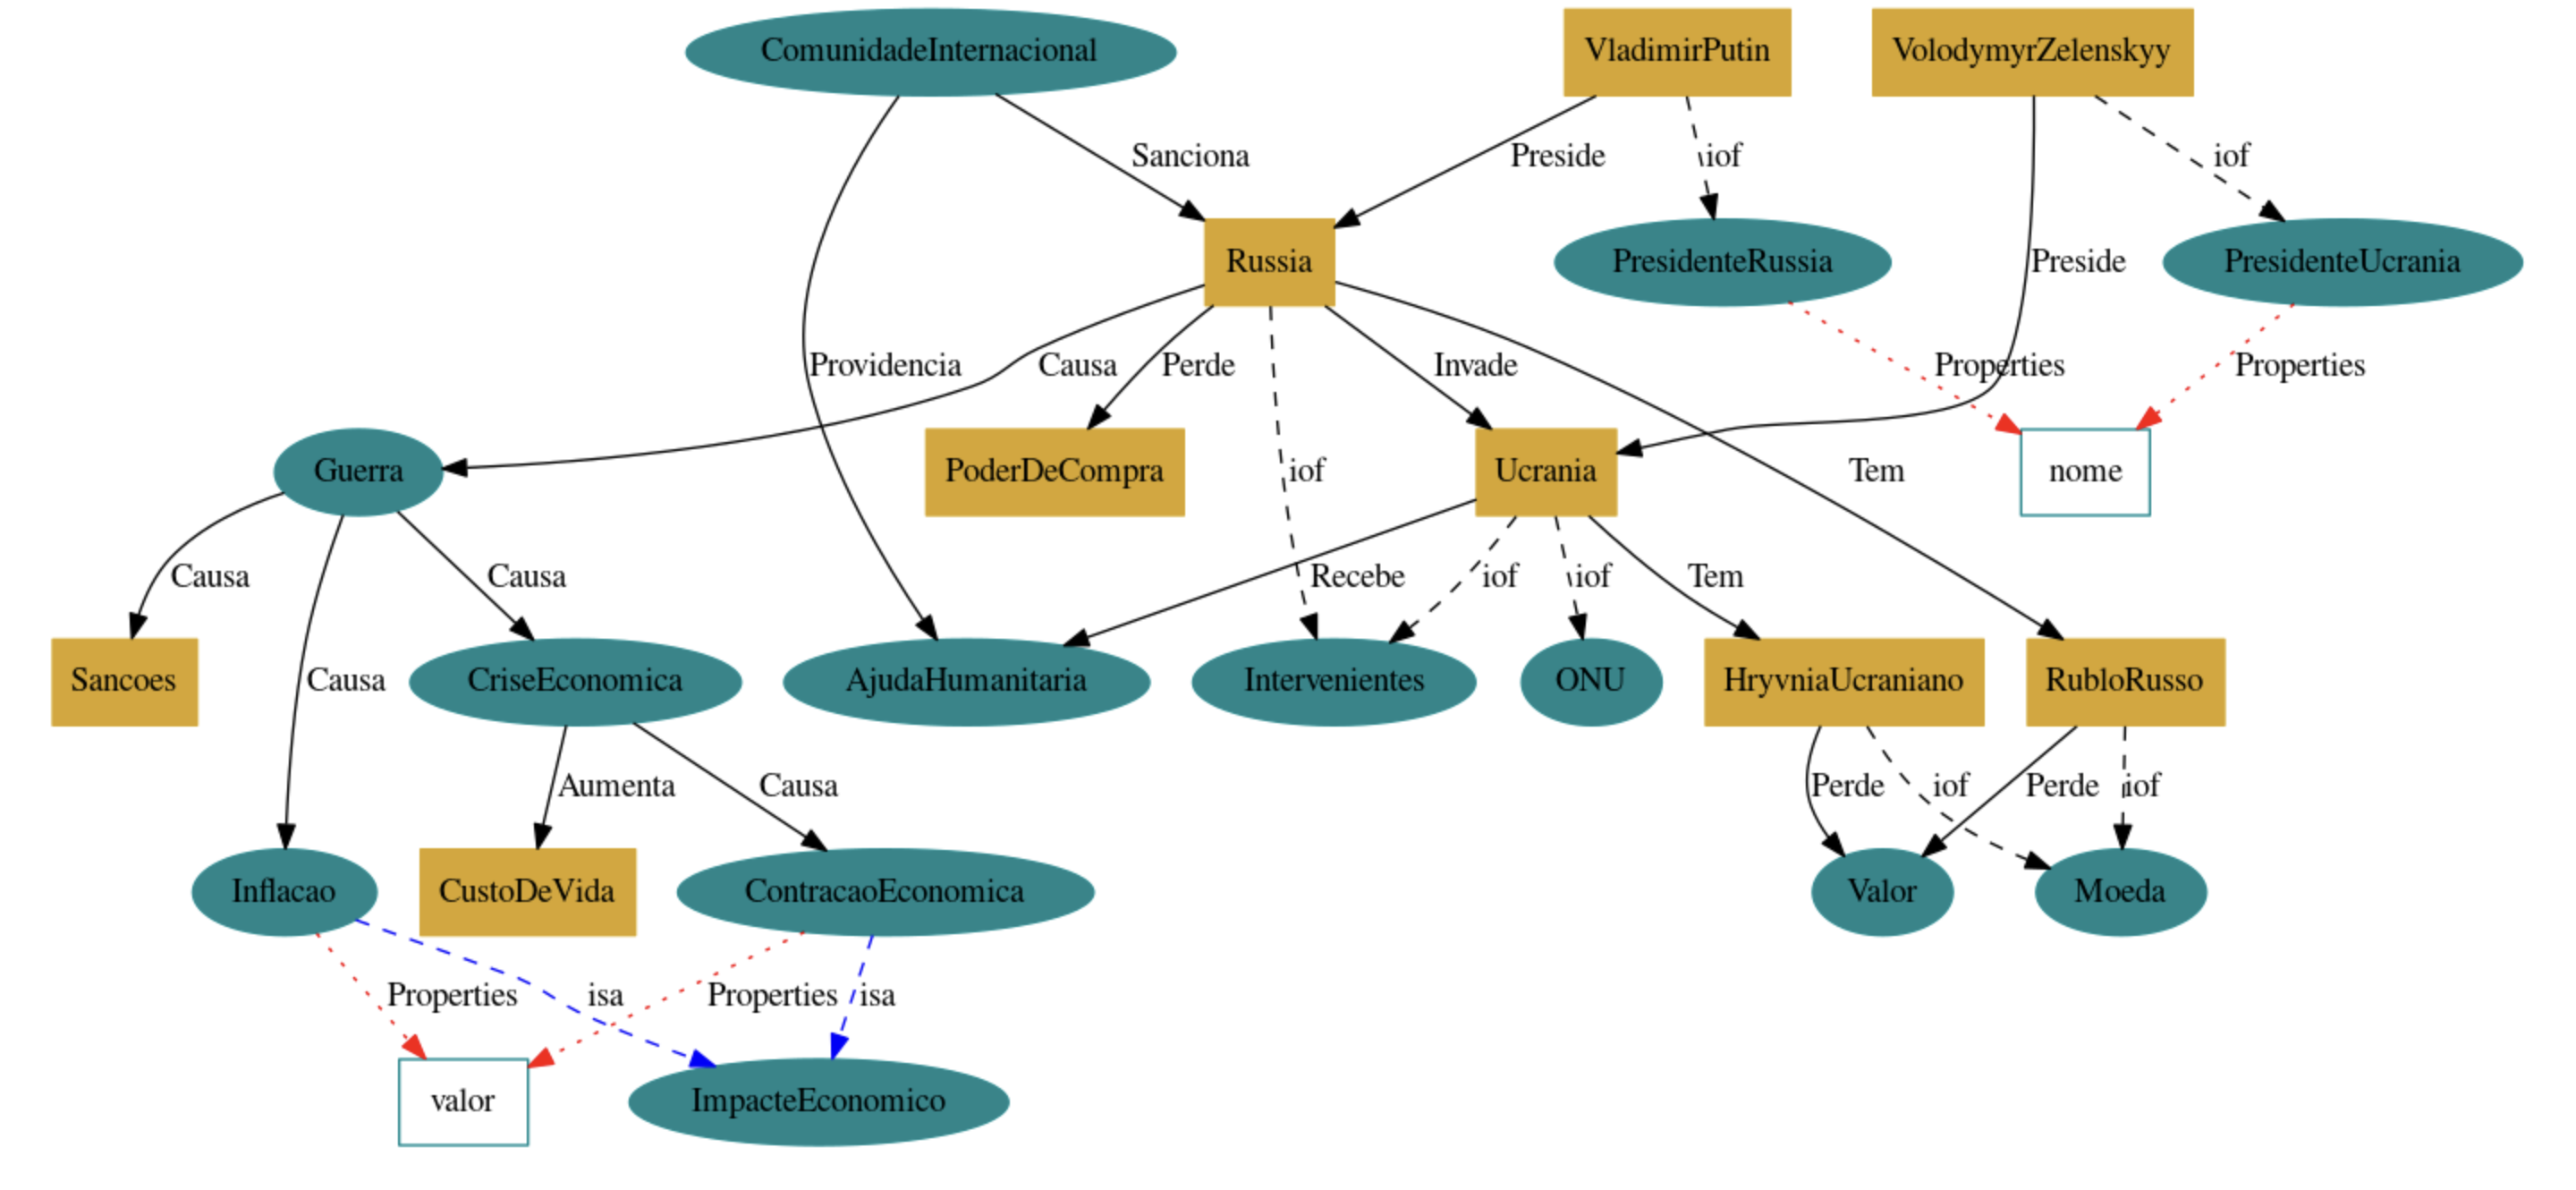
\includegraphics[width=1.2\textwidth, angle=90]{Screenshot 2023-05-24 at 19.04.46.png}
    \caption{\textbf{Ontologia-} A guerra na Ucrânia e a sua vertente económica.}
    \label{fig:my_label}
\end{figure}


\chapter{Conclusão}
\section{Considerações finais e Conclusão:}
{O trabalho realizado pelo grupo contribuiu para consolidar os conhecimentos adquiridos no âmbito desta Unidade Curricular e permitiu que os seus elementos aplicassem esses mesmos conhcimentos adquiridos de forma prática. Também é de particular ênfase a cultura geral e a consciencialização sobre o evento bélico em curso que este trabalho proporcionou aos elementos que o elaboraram.


\chapter{Bibliografia}
{Lloyd, N.; Rocher, M. e Weinert, F.. (2022, Junho 08), O impacto da guerra na Ucrânia na Economia Europeia, \textit{euronews.}, https://pt.euronews.com/next/ \\ 2022/06/08/o-impacto-da-guerra-na-ucrania-na-economia-europeia


Sondagem: Portugueses reduzem despesas mas nao querem que a Ucrania ceda na guerra 


DN/Lusa. (2022, junho 15). Portugueses entre os mais alarmados com impacto da guerra no custo de vida. \textit{Diário de Notícias}. https://www.dn.pt/ \\ internacional/portugueses-entre-os-mais-alarmados-com-impacto-da-guerra-no-custo-de-vida-14944518.html



guerra e crise economica criam mais 4 milhoes de criancas pobres, diz Unicef<



Lusa e SIC Notícias. (2023, fevereiro 14). Um ano de guerra na Ucrânia: inflação no pico das últimas décadas devido à crise energética. \textit{SIC Notícias}. https://sicnoticias.pt/especiais/guerra-russia-ucrania/2023-02-14-Um-ano-de-guerra-na-Ucrania-inflacao-no-pico-das-ultimas-decadas-devido-a-crise \\ -energetica-ba073a7e


Laja, R. (2023, fevereiro 21). Sanções, \\ crise energética e preços que não vão descer. Qual o preço de um ano de guerra na Europa?. \textit{CNN Portugal}. https://cnnportugal.iol.pt/guerra/ucrania \\ /sancoes-crise-energetica-e-precos-que-nao-vao-descer-qual-o-preco-de-um-ano-de-guerra-na-europa/20230221 \\ /63ee4a4a0cf2665294d5dc0b

Carter, B. (2023, março 08). Com ajuda da UE, economia ucraniana resiste à guerra. \textit{euronews.}. https://pt.euronews.com/next/2023/03/08/com-ajuda-da-ue-economia-ucraniana-resiste-a-guerra

M. Lourenço, S. (2023. fevereiro 23). Guerra na Ucrânia vai deixar marcas permanentes na economia da Europa. \textit{Expresso}. https://expresso.pt/economia\\/2023-02-23-Guerra-na-Ucrania-vai-deixar-marcas-permanentes-na-economia-da-Europa-a2596f18

Horowitz, J. (2023, março 09). Guerra na Ucrânia terá consequências "bastante devastadoras" para a economia da Rússia - e o aviso não é de qualquer um. \textit{CNN Portugal}. https://cnnportugal.iol.pt/fmi/russia/fmi-diz-que-guerra-na-ucrania-tera-consequencias-bastante-devastadoras-para-a-economia-da-russia/20230309/640932380cf2c84d7fcb8e68

Lloyd, N. (2022, junho 08). Como é que a economia da Europa foi afetada pela guerra da Rússia na Ucrânia?. \textit{euronews.}. https://pt.euronews.com/next\\/2022/06/08/como-e-que-a-economia-da-europa-foi-afetada-pela-guerra-da-russia-na-ucrania

Aníbal, S.; Ferreira, V; Burd Relvas, R; Villalobos, L e Aveiro, I. (2022, fevereiro 25). Que efeitos terá a guerra na economia?. \textit{PÚBLICO}. \\ https://www.publico.pt/2022/02/25/economia/noticia/efeitos-tera-guerra-economia-1996742

Guerreiro Rodrigues, J. (2023, abril 16). A economia russa resiste, mas até quando? Putin arranja formas cada vez mais originais de contornar as sanções. \textit{CNN Portugal}.  https://cnnportugal.iol.pt/russia/guerra/a-economia-russa-resiste-mas-ate-quando-putin-arranja-formas-cada-vez-mais-originais-de-contornar-as-sancoes/20230416/643588900cf2c84d7fd0e22d

Filpe, C. (2022, novembro 27). Sondagem: Portugueses reduzem despesas mas não querem que a Ucrânia ceda na guerra. \textit{Jornal de Negócios. } https://www.jornaldenegocios.pt/economia/detalhe/sondagem-portugueses-reduzem-despesas-mas-nao-querem-que-a-ucrania-ceda-na-guerra
}

DN/ Lusa. (2022, outubro 17). Guerra e crise económica criam mais 4 milhões de crianças pobres, diz Unicef. \textit{Diário de Notícias}. https://www.dn.pt\\/internacional/guerra-e-crise-economica-criam-mais-4-milhoes-de-criancas-pobres-diz-unicef-15260441.html
\end{document}